\chapter{Efficient model utilization}



\section{Low-rank adaptation} \label{sec:lora}

\begin{description}
    \item[Low-rank adaptation (LoRA)] \marginnote{Low-rank adaptation (LoRA)}
        Method to update weights by learning an offset that uses fewer parameters.

        Consider a weight matrix $\matr{W} \in \mathbb{R}^{d \times k}$, LoRA decomposes the update into two learnable matrices $\matr{A} \in \mathbb{R}^{d \times r}$ and $\matr{B} \in \mathbb{R}^{r \times k}$ (with $r \ll d, k$). Weights update is performed as:
        \[ \matr{W}_{\text{fine-tuned}} = \matr{W}_{\text{pre-trained}} + \matr{AB} \]

        \begin{figure}[H]
            \centering
            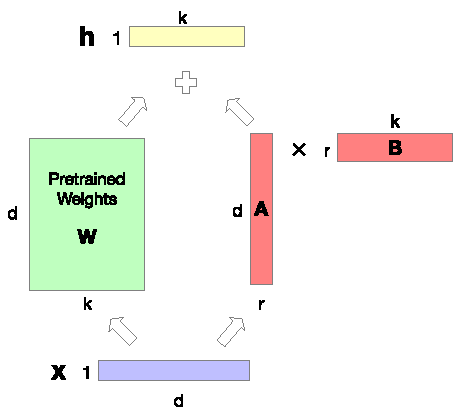
\includegraphics[width=0.4\linewidth]{./img/_lora.pdf}
        \end{figure}
\end{description}



\section{Model compression}


\subsection{Parameters compression}

\begin{description}
    \item[Parameter sharing] \marginnote{Parameter sharing}
        Use the same parameters between layers.

    \item[Pruning] \marginnote{Pruning}
        Remove weights with small impact on the loss.

        \begin{remark}
            Dropping some weights produce sparse matrices that are unoptimized for parallel hardware. Therefore, this approach does not always improve efficiency.
        \end{remark}

    \item[Quantization] \marginnote{Quantization}
        Store and perform operations with lower precision floating-points (e.g., FP32 to FP4).
\end{description}


\subsection{Training compression}

\begin{description}
    \item[Mixture of experts] \marginnote{Mixture of experts}
        Specialize smaller models on subsets of data and train a router to forward the input to the correct expert.

        \begin{remark}
            This approach can be easily deployed on distributed systems.
        \end{remark}

    \item[Knowledge distillation] \marginnote{Knowledge distillation}
        Train a student model to emulate the teacher's hidden states. In a general setting, the output distribution of the teacher is used to create the student. Two losses are used:
        \begin{descriptionlist}
            \item[Distillation loss] 
                Matches the output distribution of the student to the one of the teacher. A softmax with higher temperature is usually used so that training contribution does not only come from the highest probability.

            \item[Student loss] 
                Matches the output distribution of the student with the ground-truth (i.e., same loss of the training task).
        \end{descriptionlist}

        \begin{figure}[H]
            \centering
            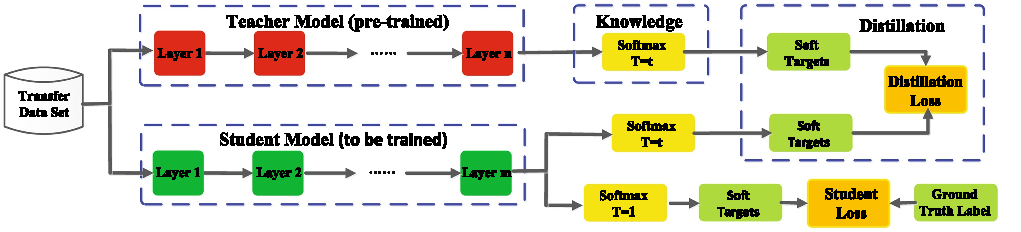
\includegraphics[width=0.8\linewidth]{./img/_distillation.pdf}
        \end{figure}

    \item[Vocabulary transfer] \marginnote{Vocabulary transfer}
        Use a domain-specific tokenizer to reduce the number of tokens to represent complex/domain-specific words and reduce the size of the embedding matrix.

        \begin{description}
            \item[Fast vocabulary transfer (FVT)] \marginnote{Fast vocabulary transfer (FVT)}
                Given:
                \begin{itemize}
                    \item A starting embedding model with tokenizer $\mathcal{T}_\text{s}$, vocabulary $V_\text{s}$, and embedding matrix $\matr{E}_\text{s}$,
                    \item A new tokenizer $\mathcal{T}_\text{dom}$ trained on a domain-specific corpus,
                \end{itemize}
                The embedding matrix $\matr{E}_\text{dom}$ for the vocabulary $V_\text{dom}$ of $\mathcal{T}_\text{dom}$ is built as follows:
                \[ 
                    \forall t_i \in V_\text{dom}: \matr{E}_\text{dom}(t_i) = \frac{1}{|\mathcal{T}_\text{s}(t_i)|} \sum_{t_j \in \mathcal{T}_\text{s}(t_i)}\matr{E}_\text{s}(t_j)
                \]
                In other words, each token in $V_\text{dom}$ is encoded as the average of the embeddings of the tokens that compose it in the starting embedding model (if the token appear in both vocabularies, the embedding is the same).
        \end{description}
\end{description}



\section{In-context learning}

\begin{description}
    \item[Prompting] \marginnote{Prompting}
        Pass a prompt to the language model to condition generation.

        More formally, a prompt is defined by means of a prompting function $f_\text{prompt}(\cdot)$ that formats an input text $x$. $f_\text{prompt}$ typically has a slot for the input and a slot for the answer (e.g., the class in case of classification). The prompt is then fed to the language model that searches the highest scoring word $\hat{z}$ to fill the answer as follows:
        \[ \hat{z} = \arg\max \prob{ f_\text{fill}(f_\text{prompt}(x), z); \theta } \]
        Where $f_\text{fill}(f_\text{prompt}(x), z)$ inserts $z$ in the prompt. In other word, we are looking for the word that makes the model least perplexed.

        \begin{example}
            A prompt for sentiment analysis of movie reviews might be:
            \begin{center}
                \texttt{[X] Overall, it was a [Z] movie.}
            \end{center}
            Where \texttt{[X]} is the placeholder for the review and \texttt{[Z]} is for the class.
        \end{example}

        \begin{remark}
            The prompt does not necessarily need to be text (i.e., discrete/hard prompts). Continuous/soft prompts (i.e., embeddings) can also be used to condition generation.
        \end{remark}


    \item[Zero-shot learning] \marginnote{Zero-shot learning}
        Solve a task by providing a language model the description of the problem in natural language.

    \item[One-shot learning] \marginnote{One-shot learning}
        Solve a task by providing a language model the description of the problem in natural language and a single demonstration (i.e., an example).

    \item[Few-shot learning] \marginnote{Few-shot learning}
        Solve a task by providing a language model the description of the problem in natural language and a few demonstrations.

        \begin{remark}
            Empirical results show that not too many examples are required. Also, too many examples might reduce performance.
        \end{remark}
\end{description}

\begin{remark}
    Some studies show that an explanation for in-context learning is that causal attention has the same effect of gradient updates (i.e., the left part of the prompt influences the right part).

    Another possible explanation is based on the concept of induction heads which are attention heads that specialize in predicting repeated sequences (i.e., in-context learning is seen as the capability of imitating past data). Ablation studies show that by identifying and removing induction heads, the in-context learning performance of a model drastically drops.

    \begin{figure}[H]
        \centering
        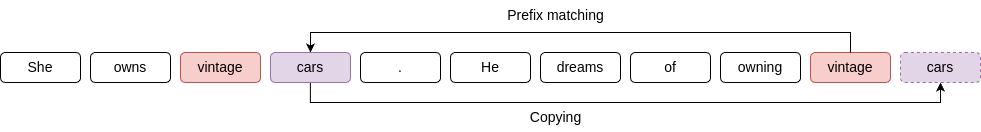
\includegraphics[width=0.9\linewidth]{./img/induction_head.png}
        \caption{Example of induction head}
    \end{figure}
\end{remark}

\begin{description}
    \item[Prefix-tuning] \marginnote{Prefix-tuning}
        Soft prompting technique that learns some prefix embeddings for a specific task to add to the prompt while keeping the rest of the model frozen.

        \begin{figure}[H]
            \centering
            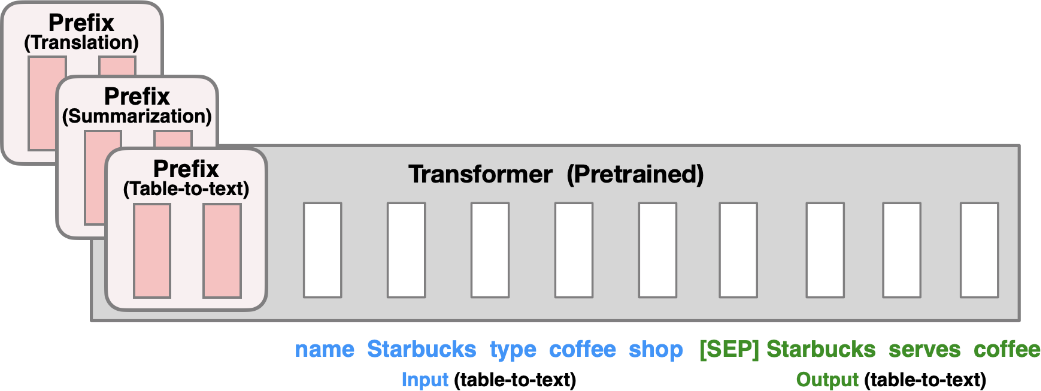
\includegraphics[width=0.65\linewidth]{./img/prefix_tuning.png}
        \end{figure}

    \item[Chain-of-thought prompting] \marginnote{Chain-of-thought prompting}
        Provide in the prompt examples of reasoning to make the model generate the output step-by-step\footnote{
\includegraphics[width=1.2cm]{img/meme.jpg}}.

        \begin{remark}
            Empirical results show that the best prompt for chain-of-thought is to add to the prompt \texttt{think step by step}.
        \end{remark}
\end{description}